\documentclass[conference,a4paper]{IEEEtran}
\IEEEoverridecommandlockouts
% ---------------------------------------------------------------
% Preámbulo: paquetes, estilos de código y macros para los diagramas UML (TikZ)
% ---------------------------------------------------------------
\usepackage[T1]{fontenc}
\usepackage[utf8]{inputenc}
\usepackage[spanish,es-noshorthands,es-tabla,es-nodecimaldot]{babel}
\usepackage{cite}
\usepackage{amsmath,amssymb}
\usepackage{graphicx}
\usepackage[table]{xcolor}
\usepackage{listings}
\usepackage{booktabs}
\usepackage{tabularx}
\usepackage{array}
\usepackage{tikz}
\usetikzlibrary{arrows.meta,positioning,shapes.geometric,shapes.multipart,fit,calc,backgrounds,babel}
\usepackage{url}
\usepackage[hidelinks]{hyperref}

\renewcommand{\IEEEkeywordsname}{Palabras clave}
\renewcommand{\lstlistingname}{Listado}
\def\UrlBreaks{\do\/\do-\do.}

% ---------- Código fuente ----------
\definecolor{fondoCodigo}{RGB}{247,248,250}
\definecolor{clave}{RGB}{0,92,170}
\definecolor{cadena}{RGB}{163,21,21}
\definecolor{comentario}{RGB}{0,128,0}
\definecolor{tipo}{RGB}{38,127,153}

\lstdefinelanguage{TypeScript}{
  keywords={abstract,as,async,await,break,case,catch,class,const,constructor,continue,declare,default,do,else,enum,
    export,extends,false,finally,for,from,function,get,if,implements,import,in,instanceof,interface,keyof,let,
    namespace,new,null,of,override,private,protected,public,readonly,return,satisfies,set,static,super,switch,this,
    throw,true,try,type,typeof,undefined,void,while},
  morekeywords=[2]{string,number,boolean,unknown,never,any,Promise,Record,Partial,Omit,Pick,Readonly,ReadonlyArray,Map},
  sensitive=true,
  morecomment=[l]{//},
  morecomment=[s]{/*}{*/},
  morestring=[b]',
  morestring=[b]",
  morestring=[b]`,
}
\lstdefinelanguage{JavaScript}{
  keywords={async,await,break,case,catch,class,const,constructor,continue,default,do,else,export,extends,false,
    finally,for,from,function,get,if,import,in,instanceof,let,new,null,of,return,set,static,super,switch,this,throw,
    true,try,typeof,undefined,void,while},
  sensitive=true,
  morecomment=[l]{//},
  morecomment=[s]{/*}{*/},
  morestring=[b]',
  morestring=[b]",
  morestring=[b]`,
}
\lstset{
  basicstyle=\ttfamily\scriptsize,
  keywordstyle=\color{clave}\bfseries,
  keywordstyle=[2]\color{tipo},
  stringstyle=\color{cadena},
  commentstyle=\color{comentario}\itshape,
  backgroundcolor=\color{fondoCodigo},
  frame=single,
  rulecolor=\color{gray!40},
  framesep=2pt,
  xleftmargin=3pt,
  xrightmargin=3pt,
  breaklines=true,
  breakatwhitespace=true,
  columns=fullflexible,
  keepspaces=true,
  showstringspaces=false,
  tabsize=2,
  captionpos=b,
  inputencoding=utf8,
  extendedchars=true,
  literate={á}{{\'a}}1 {é}{{\'e}}1 {í}{{\'i}}1 {ó}{{\'o}}1 {ú}{{\'u}}1 {ñ}{{\~n}}1
           {Á}{{\'A}}1 {É}{{\'E}}1 {Í}{{\'I}}1 {Ó}{{\'O}}1 {Ú}{{\'U}}1 {Ñ}{{\~N}}1
           {¿}{{?`}}1 {¡}{{!`}}1,
}

% ---------- Macros UML (TikZ) ----------
\newcommand{\estereotipo}[1]{\guillemotleft #1\guillemotright}

% Actor (monigote). #1 nombre, #2 posición "x,y", #3 etiqueta.
% Define las coordenadas #1-e (este), #1-o (oeste) y el nodo #1-etq (etiqueta).
\newcommand{\actorUML}[3]{%
  \begin{scope}[shift={(#2)}]
    \draw[thick] (0,0.62) circle (0.17);
    \draw[thick] (0,0.45) -- (0,-0.05);
    \draw[thick] (-0.32,0.28) -- (0.32,0.28);
    \draw[thick] (0,-0.05) -- (-0.24,-0.5);
    \draw[thick] (0,-0.05) -- (0.24,-0.5);
    \node[below, font=\small, inner sep=2pt] (#1-etq) at (0,-0.52) {#3};
    \coordinate (#1-e) at (0.42,0.2);
    \coordinate (#1-o) at (-0.42,0.2);
  \end{scope}}

% Icono de componente UML en la esquina superior derecha de un nodo
\newcommand{\iconoComponente}[1]{%
  \draw[fill=white] ($(#1.north east)+(-0.40,-0.10)$) rectangle ++(0.26,-0.30);
  \draw[fill=white] ($(#1.north east)+(-0.46,-0.15)$) rectangle ++(0.12,-0.06);
  \draw[fill=white] ($(#1.north east)+(-0.46,-0.27)$) rectangle ++(0.12,-0.06);}

% Estilos de los diagramas de clases
\tikzset{
  clases/.style={
    clase/.style={draw, thick, fill=white, anchor=north, rectangle split, rectangle split parts=3,
      rectangle split part fill={teal!14,white,white}, text width=3.4cm, align=left,
      font=\scriptsize, inner sep=2.5pt, execute at begin node={\setlength{\parindent}{0pt}}},
    interfaz/.style={clase, rectangle split parts=2, rectangle split part fill={orange!14,white}},
    simple/.style={clase, rectangle split parts=2, rectangle split part fill={teal!14,white}},
    herencia/.style={thick, -{Triangle[open, length=2.6mm, width=2.6mm]}},
    realiza/.style={dashed, -{Triangle[open, length=2.6mm, width=2.6mm]}},
    asociacion/.style={-{Stealth[length=2mm]}},
    depende/.style={dashed, -{Stealth[length=2mm]}},
    composicion/.style={{Diamond[length=3mm, width=2mm]}-},
    agregacion/.style={{Diamond[open, length=3mm, width=2mm]}-},
    rol/.style={font=\tiny, inner sep=1pt},
  },
}
% \clase{nombre}{x,y}{encabezado}{atributos}{métodos}
\newcommand{\clase}[5]{\node[clase] (#1) at (#2)
  {{\centering #3\par}\nodepart{two}{\raggedright #4\par}\nodepart{three}{\raggedright #5\par}};}
% \interfaz / \simple {nombre}{x,y}{encabezado}{cuerpo}
\newcommand{\interfaz}[4]{\node[interfaz] (#1) at (#2) {{\centering #3\par}\nodepart{two}{\raggedright #4\par}};}
\newcommand{\simple}[4]{\node[simple] (#1) at (#2) {{\centering #3\par}\nodepart{two}{\raggedright #4\par}};}


\begin{document}

\title{Migración a TypeScript de FamiFinanzas: aplicación web para la gestión del presupuesto familiar\thanks{Taller TypeScript --- Electiva II (60) 8108277, periodo académico II-2026. Universidad Pedagógica y Tecnológica de Colombia.}}

\author{
\IEEEauthorblockN{Samuel Salamanca}
\IEEEauthorblockA{\textit{Escuela de Ingeniería de Sistemas y Computación}\\
\textit{Universidad Pedagógica y Tecnológica de Colombia}\\
Tunja, Colombia}
\and
\IEEEauthorblockN{Rafael Cristancho}
\IEEEauthorblockA{\textit{Escuela de Ingeniería de Sistemas y Computación}\\
\textit{Universidad Pedagógica y Tecnológica de Colombia}\\
Tunja, Colombia}
}

\maketitle

\begin{abstract}
Este documento describe la migración a TypeScript de FamiFinanzas, la aplicación web de gestión de gastos, ingresos y presupuesto familiar desarrollada en el Taller~2 del primer corte con Node.js, Express, EJS, JWT y SQLite. La migración abarcó tres frentes: (i) la reestructuración del modelo en una jerarquía de clases con interfaces, clases abstractas, genéricos, enumeraciones y encapsulamiento; (ii) el reemplazo de todos los scripts JavaScript del backend por archivos \texttt{.ts} transpilados con \texttt{tsc} a JavaScript limpio en la carpeta \texttt{dist/}; y (iii) un nuevo frontend escrito en TypeScript que se transpila a módulos ES nativos (\texttt{public/js/*.js}) y agrega validación en vivo, simulación del presupuesto, un gráfico interactivo y tablas ordenables. Los contratos de datos (DTO) se comparten entre servidor y cliente mediante un archivo de declaraciones, de modo que un cambio en la API se detecta en tiempo de compilación en ambos lados. La API REST conserva su comportamiento: las 29 pruebas de integración originales pasan sin modificar su lógica, junto con 12 pruebas nuevas, y el rendimiento se mantiene por debajo de 10\,ms (p95) con 10\,000 gastos.
\end{abstract}

\begin{IEEEkeywords}
TypeScript, migración de software, programación orientada a objetos, Node.js, Express, transpilación, UML.
\end{IEEEkeywords}

% =====================================================================
\section{Introducción}
JavaScript es el lenguaje de la web, pero su tipado dinámico traslada a tiempo de ejecución errores que podrían detectarse antes: propiedades mal escritas, parámetros con la forma equivocada o valores \texttt{undefined} que se propagan. Gao, Bird y Barr estimaron que un sistema de tipos estático como el de TypeScript habría detectado cerca del 15\,\% de los errores públicos analizados en proyectos JavaScript \cite{gao2017}. TypeScript es un superconjunto de JavaScript que agrega anotaciones de tipo opcionales, interfaces, genéricos y modificadores de acceso, y que se transpila a JavaScript estándar \cite{tshandbook,bierman2014}.

En el Taller~2 se construyó \emph{FamiFinanzas}, una aplicación web para que una familia registre sus gastos e ingresos, defina presupuestos mensuales por categoría y reciba alertas al alcanzar el 80\,\% y el 100\,\% de cada presupuesto. El objetivo de este taller es migrar esa aplicación a TypeScript, aprovechando la migración para resaltar las ventajas del lenguaje: un modelo orientado a objetos explícito, backend tipado de extremo a extremo y vistas del cliente implementadas en TypeScript.

El documento se organiza así: la Sección~\ref{sec:base} resume el sistema de partida; la Sección~\ref{sec:proceso} describe el proceso de migración con fragmentos comparativos de código JavaScript y TypeScript; la Sección~\ref{sec:uml} presenta los modelos UML; la Sección~\ref{sec:resultados} reporta la verificación y la Sección~\ref{sec:conclusiones} concluye.

% =====================================================================
\section{Sistema de partida (Taller 2)}\label{sec:base}
FamiFinanzas expone una API REST versionada (\texttt{/api/v1}) documentada con OpenAPI/Swagger y protegida con JSON Web Tokens (JWT) \cite{rfc7519}, además de un front-end renderizado en el servidor con plantillas EJS que guarda el mismo JWT en una cookie \emph{httpOnly}. La persistencia usa el módulo \texttt{node:sqlite} de Node.js 22 \cite{nodesqlite} y la validación de entradas la biblioteca Zod \cite{zod}. La arquitectura sigue capas: rutas (controladores), servicios (reglas de negocio), repositorios (SQL parametrizado) y base de datos. La Tabla~\ref{tab:rf} resume los requisitos funcionales, que la migración conserva íntegramente.

\begin{table}[!t]
\centering
\caption{Requisitos funcionales de FamiFinanzas}
\label{tab:rf}
\footnotesize
\begin{tabularx}{\columnwidth}{@{}lX@{}}
\toprule
\textbf{ID} & \textbf{Requisito} \\
\midrule
RF-01 & Registrar familia, administrador y 8 categorías iniciales \\
RF-02 & Iniciar sesión con correo y contraseña; emitir JWT (2\,h) \\
RF-03 & Gestionar miembros de la familia (administrador) \\
RF-04 & Gestionar categorías; desactivar si tienen gastos \\
RF-05/06/07 & Registrar, filtrar/paginar y editar/eliminar gastos \\
RF-08 & Gestionar ingresos \\
RF-09 & Definir presupuestos mensuales por categoría \\
RF-10 & Alertar al 80\,\% y al superar el presupuesto \\
RF-11 & Resumen mensual por categoría y por miembro \\
RF-12 & Exportar gastos filtrados a CSV \\
RF-13 & Consultar perfil y cambiar contraseña \\
RF-14 & Autorización por rol y aislamiento entre familias \\
\bottomrule
\end{tabularx}
\end{table}

El código JavaScript original tenía limitaciones que motivaron la migración: los repositorios y servicios eran objetos literales con lógica duplicada (por ejemplo, \texttt{gastoService} e \texttt{ingresoService} repetían \texttt{obtener} y \texttt{eliminar}); la clase abstracta \texttt{Movimiento} existía en el diagrama de clases pero no en el código; los estados (\texttt{'ADMIN'}, \texttt{'EXCEDIDO'}\ldots) eran cadenas sueltas; y el hash de la contraseña se ocultaba ``de memoria'' con una función \texttt{sinHash}. El frontend era un único archivo \texttt{app.js} de 25 líneas.

% =====================================================================
\section{Proceso de migración}\label{sec:proceso}
\subsection{Estrategia}
La migración se ejecutó de forma incremental y guiada por las pruebas existentes, en cinco fases:
\begin{enumerate}
\item \textbf{Configuración}: instalación de \texttt{typescript} y de las definiciones \texttt{@types/*}, y creación de dos proyectos de compilación (backend y cliente) que comparten un \texttt{tsconfig.base.json}.
\item \textbf{Contratos}: definición de los DTO de la API en \texttt{src/shared/contratos.d.ts}.
\item \textbf{Dominio}: creación de la jerarquía de clases (Sección~\ref{sec:jerarquia}).
\item \textbf{Backend}: conversión de configuración, base de datos, repositorios, servicios, middlewares y rutas a \texttt{.ts}.
\item \textbf{Frontend}: implementación de las vistas del cliente en TypeScript (\texttt{client/}).
\end{enumerate}
El código JavaScript original se conservó en \texttt{legacy-js/} como referencia para la comparación.

\subsection{Configuración del compilador}
El Listado~\ref{lst:tsconfig} muestra la configuración común. Se activó el modo \texttt{strict} (incluye \texttt{strictNullChecks} y \texttt{noImplicitAny}), \texttt{noImplicitOverride} para exigir la palabra \texttt{override} al sobrescribir métodos y \texttt{verbatimModuleSyntax}, que obliga a importar los tipos con \texttt{import type} para que el JavaScript generado no contenga importaciones innecesarias. El backend usa \texttt{module: NodeNext} y emite en \texttt{dist/}; el cliente usa \texttt{module: ES2022}, las bibliotecas \texttt{DOM} y emite en \texttt{public/js/} \cite{tsconfig}.

\begin{lstlisting}[language=TypeScript, caption={tsconfig.base.json (opciones comunes) y diferencias por proyecto}, label={lst:tsconfig}]
{ "compilerOptions": {
    "target": "ES2022", "strict": true,
    "noImplicitOverride": true, "noImplicitReturns": true,
    "noUnusedLocals": true, "noUnusedParameters": true,
    "isolatedModules": true, "verbatimModuleSyntax": true,
    "sourceMap": true } }
// tsconfig.json (backend):  module NodeNext, lib ES2022,
//   rootDir ".", outDir "dist"   -> dist/src, dist/tests
// tsconfig.client.json:     module ES2022, lib DOM,
//   rootDir "client", outDir "public/js"
\end{lstlisting}

Los \emph{scripts} de \texttt{npm} quedaron así: \texttt{build} ejecuta ambos proyectos; \texttt{start} compila (\texttt{prestart}) y arranca \texttt{node dist/src/server.js}; \texttt{test} compila y ejecuta las pruebas transpiladas con el ejecutor nativo \texttt{node --test}; \texttt{typecheck} verifica tipos sin emitir archivos.

\subsection{Jerarquía de clases y elementos de POO}\label{sec:jerarquia}
Los modelos se reescribieron como clases (Fig.~\ref{fig:clases-dominio}). La raíz es la clase abstracta genérica \texttt{Entidad<TDTO>}, que fija el identificador inmutable y obliga a cada subclase a implementar \texttt{toJSON()} con la forma exacta de su DTO. \texttt{Movimiento<TDTO>}, que en JavaScript solo existía en el diagrama, es ahora una clase abstracta de la que heredan \texttt{Gasto} e \texttt{Ingreso}; contiene la regla de propiedad RF-07 (\texttt{puedeSerModificadoPor}) y el método abstracto \texttt{tipo}, resuelto por polimorfismo. Se definieron las interfaces \texttt{Serializable}, \texttt{Modificable}, \texttt{ExportableCsv} y \texttt{Actor}; las enumeraciones \texttt{Rol}, \texttt{MetodoPago} y \texttt{EstadoPresupuesto}; y el objeto de valor inmutable \texttt{EjecucionPresupuesto}, con constructor privado y método de fábrica estático, que reemplaza a la función suelta \texttt{estadoPresupuesto()}.

El encapsulamiento se reforzó con los campos privados de ECMAScript \cite{ecma262}: el hash de la contraseña de \texttt{Usuario} es \texttt{\#passwordHash}, por lo que no aparece en \texttt{JSON.stringify}, en el operador de propagación ni en \texttt{Object.keys} (Listado~\ref{lst:usuario}). Los errores se modelaron como jerarquía (Fig.~\ref{fig:clases-err}a): cada subclase de \texttt{AppError} fija su código HTTP, lo que elimina códigos escritos a mano (Fig.~\ref{fig:cmp-errores}).

\begin{lstlisting}[language=TypeScript, caption={Encapsulamiento con campo privado y tipos de enumeración}, label={lst:usuario}]
export class Usuario extends Entidad<UsuarioDTO>
                     implements Actor {
  readonly rol: Rol;                // enum, no string
  readonly #passwordHash: string | undefined;
  get hashContrasena() { return this.#passwordHash; }
  esAdmin(): boolean { return this.rol === Rol.ADMIN; }
  override toJSON(): UsuarioDTO { /* sin el hash */ }
}
// Record<Enum, string> exige una etiqueta por cada valor:
export const NOMBRES_METODO: Readonly<Record<MetodoPago,
  string>> = { [MetodoPago.EFECTIVO]: 'Efectivo', ... };
\end{lstlisting}

\begin{figure*}[!t]
\centering
\begin{minipage}[t]{0.47\textwidth}
\begin{lstlisting}[language=JavaScript, title={\textbf{Antes (JS)} --- src/utils/errores.js}]
export class AppError extends Error {
  constructor(status, codigo, mensaje, detalles) {
    super(mensaje);
    this.status = status;
    this.codigo = codigo;
    this.detalles = detalles;
  }
}
export const noEncontrado = (recurso) =>
  new AppError(404, 'NO_ENCONTRADO',
               `${recurso} no encontrado`);
export const conflicto = (mensaje) =>
  new AppError(409, 'CONFLICTO', mensaje);
// En otro servicio, el código se repetía a mano:
throw new AppError(409, 'CONFLICTO', 'La familia...');
\end{lstlisting}
\end{minipage}\hfill
\begin{minipage}[t]{0.5\textwidth}
\begin{lstlisting}[language=TypeScript, title={\textbf{Después (TS)} --- src/utils/errores.ts}]
export class AppError extends Error {
  constructor(
    readonly status: number,
    readonly codigo: string,
    mensaje: string,
    readonly detalles?: DetalleErrorDTO[],
  ) {
    super(mensaje);
    this.name = new.target.name;
  }
  aRespuesta(): ErrorApiDTO { ... }
}
export class NoEncontradoError extends AppError {
  constructor(recurso: string) {
    super(404, 'NO_ENCONTRADO', `${recurso} no encontrado`);
  }
}
export class ConflictoError extends AppError { ... }
\end{lstlisting}
\end{minipage}
\caption{Snapshot comparativo de la migración de los errores: de funciones fábrica a una jerarquía de clases con propiedades de parámetro \texttt{readonly}.}
\label{fig:cmp-errores}
\end{figure*}

\subsection{Backend: reemplazo de los scripts JavaScript}
Los 25 archivos \texttt{.js} de \texttt{src/} se reemplazaron por archivos \texttt{.ts}. Los cambios más representativos fueron:

\textbf{Repositorios genéricos.} Se creó la clase abstracta \texttt{RepositorioBase<TEntidad, TFila>} (patrón \emph{Repository} \cite{fowler2002}) que centraliza el acceso a \texttt{node:sqlite} y exige implementar \texttt{mapear(fila)}. Cada tabla declara la interfaz de su fila (\texttt{FilaGasto}, en \emph{snake\_case}) y el repositorio devuelve objetos de dominio. Gastos e ingresos comparten \texttt{MovimientoRepository<T, TFila>}, que implementa una sola vez los filtros por fecha y miembro, la paginación y el aislamiento por familia; \texttt{GastoRepository} solo agrega el filtro por categoría sobrescribiendo un método \emph{gancho} (Fig.~\ref{fig:cmp-repo}).

\textbf{Servicios con herencia e inyección de dependencias.} \texttt{MovimientoService<T, R>} es abstracta y genérica; \texttt{GastoService} e \texttt{IngresoService} heredan \texttt{listar}, \texttt{obtener}, \texttt{eliminar} y \texttt{verificarPropiedad}. Todas las dependencias se reciben por el constructor y se conectan en una raíz de composición (\texttt{contenedor.ts}), lo que eliminó las importaciones circulares entre servicios de la versión JavaScript.

\begin{figure*}[!t]
\centering
\begin{minipage}[t]{0.47\textwidth}
\begin{lstlisting}[language=JavaScript, title={\textbf{Antes (JS)} --- gastoRepository.js}]
const mapear = (g) => g && {
  id: g.id, monto: g.monto, fecha: g.fecha,
  metodoPago: g.metodo_pago,
  categoria: { id: g.categoria_id, ... },
  usuario: { id: g.usuario_id, ... },
};
function filtros(familiaId, { desde, hasta,
                 categoriaId, usuarioId }) { ... }
export const gastoRepository = {
  buscar(id, familiaId) {
    return mapear(db.prepare(`${SELECT} WHERE ...`)
                    .get(id, familiaId));
  },
  listar(familiaId, f) { ... },   // duplicado en
  eliminar(id, familiaId) { ... },// ingresoRepository
};
\end{lstlisting}
\end{minipage}\hfill
\begin{minipage}[t]{0.5\textwidth}
\begin{lstlisting}[language=TypeScript, title={\textbf{Después (TS)} --- GastoRepository.ts}]
interface FilaGasto {
  id: number; monto: number; fecha: string;
  metodo_pago: MetodoPago; categoria_id: number; ...
}
export class GastoRepository
    extends MovimientoRepository<Gasto, FilaGasto> {
  protected override readonly tabla = 'gastos';
  protected override readonly alias = 'g';
  protected override mapear(g: FilaGasto): Gasto {
    return new Gasto({ id: g.id, monto: g.monto, ... });
  }
  protected override filtrosAdicionales(
      { categoriaId }: CriteriosMovimiento): ClausulaWhere {
    return categoriaId ? { where: 'g.categoria_id = ?',
      params: [categoriaId] } : { where: '', params: [] };
  }
  // buscar, listar, listarTodos y eliminar se heredan
}
\end{lstlisting}
\end{minipage}
\caption{Snapshot comparativo de un repositorio: de objeto literal sin tipos a clase que hereda de un repositorio genérico. La propiedad \texttt{tabla} solo admite \texttt{'gastos' | 'ingresos'} (tipo unión de literales).}
\label{fig:cmp-repo}
\end{figure*}

\textbf{Validación y tipos inferidos.} Los esquemas Zod se mantuvieron, pero ahora reutilizan los \texttt{enum} del dominio (\texttt{z.nativeEnum}) y de ellos se derivan los tipos con \texttt{z.infer}; la función \texttt{validar} es genérica y su tipo de retorno se deduce del esquema (Listado~\ref{lst:zod}). Así, la validación en ejecución y el tipo estático nunca se desincronizan.

\begin{lstlisting}[language=TypeScript, caption={Tipos derivados de la validación y validador genérico}, label={lst:zod}]
export type EntradaGasto = z.infer<typeof esquemas.gasto>;
// { monto: number; fecha: string; categoriaId: number;
//   descripcion: string; metodoPago: MetodoPago }
export function validar<E extends z.ZodTypeAny>(
    esquema: E, datos: unknown): z.output<E> { ... }
const datos = validar(esquemas.gasto, req.body);
gastoService.crear(actor(req), datos); // EntradaGasto
\end{lstlisting}

\textbf{Express tipado.} Se amplió el tipo \texttt{Request} de Express mediante \emph{module augmentation} para declarar \texttt{req.usuario}, y la función \texttt{actor(req)} devuelve el usuario autenticado o lanza un 401, en lugar de propagar un \texttt{undefined} silencioso. Para el front-end EJS se definió la interfaz \texttt{Vistas}, que asocia cada plantilla con los datos que necesita; la función genérica \texttt{renderizar<K extends keyof Vistas>} hace que olvidar una variable de la vista sea un error de compilación (Listado~\ref{lst:vistas}). Las respuestas usan el operador \texttt{satisfies} para comprobar que cumplen el contrato sin perder el tipo inferido.

\begin{lstlisting}[language=TypeScript, caption={Ampliación de Express y render tipado de vistas EJS}, label={lst:vistas}]
declare global { namespace Express {
  interface Request { usuario?: Usuario } } }
export interface Vistas {
  'pages/login': Base & { aviso: string | null;
                          error: string | null; email: string };
  'pages/gastos': Base & { resultado: Pagina<Gasto>;
      filtro: FiltroMovimientos; qs: string; ... };
}
export function renderizar<K extends keyof Vistas>(
  res: Response, vista: K, datos: Vistas[K], status = 200) {...}
\end{lstlisting}

Durante la conversión el compilador reportó, por ejemplo, que el arreglo construido para \texttt{URLSearchParams} era \texttt{string[][]} y no la tupla \texttt{[string, string][]} que exige la API del DOM; en JavaScript ese tipo de inconsistencias pasa desapercibido hasta que falla en producción:
\begin{lstlisting}[basicstyle=\ttfamily\tiny]
src/routes/web.ts(94,23): error TS2345: Argument of type 'string[][]'
  is not assignable to parameter of type ... Iterable<[string, string]>
\end{lstlisting}

\subsection{Proceso de transpilación}
El comando \texttt{npm run build} invoca a \texttt{tsc} dos veces. Para el backend, cada archivo \texttt{src/**/*.ts} produce un \texttt{dist/src/**/*.js} con su \emph{source map}; para el cliente, \texttt{client/**/*.ts} produce \texttt{public/js/**/*.js}. Al apuntar a ES2022, el JavaScript generado conserva las clases, los campos de clase y los campos privados nativos; solo se eliminan las anotaciones de tipo, las interfaces, los modificadores \texttt{private}/\texttt{readonly}/\texttt{override} y las importaciones de solo tipos. El resultado es código limpio y legible (Fig.~\ref{fig:transpilacion}). Los archivos \texttt{.d.ts} (contratos y ampliación de Express) no generan JavaScript.

\begin{figure*}[!t]
\centering
\begin{minipage}[t]{0.5\textwidth}
\begin{lstlisting}[language=TypeScript, title={\textbf{Fuente} --- src/dominio/Gasto.ts}]
import { Movimiento, type DatosMovimiento,
         type TipoMovimiento } from './Movimiento.js';
import type { MetodoPago } from './enums.js';
import type { ExportableCsv } from './interfaces.js';
import type { GastoDTO, ReferenciaCategoriaDTO }
  from '../shared/contratos.js';

export class Gasto extends Movimiento<GastoDTO>
                   implements ExportableCsv {
  static readonly ENCABEZADO_CSV = ['ID', 'Fecha', ...] as const;
  readonly metodoPago: MetodoPago;
  readonly categoria: ReferenciaCategoriaDTO;
  constructor(datos: DatosGasto) {
    super(datos);
    this.metodoPago = datos.metodoPago;
    this.categoria = datos.categoria;
  }
  override get tipo(): TipoMovimiento { return 'GASTO'; }
  override toJSON(): GastoDTO {
    return { ...this.camposBase(),
             metodoPago: this.metodoPago,
             categoria: this.categoria };
  }
}
\end{lstlisting}
\end{minipage}\hfill
\begin{minipage}[t]{0.47\textwidth}
\begin{lstlisting}[language=JavaScript, title={\textbf{Transpilado por tsc} --- dist/src/dominio/Gasto.js}]
import { Movimiento } from './Movimiento.js';

export class Gasto extends Movimiento {
  static ENCABEZADO_CSV = ['ID', 'Fecha', ...];
  metodoPago;
  categoria;
  constructor(datos) {
    super(datos);
    this.metodoPago = datos.metodoPago;
    this.categoria = datos.categoria;
  }
  get tipo() {
    return 'GASTO';
  }
  toJSON() {
    return { ...this.camposBase(),
             metodoPago: this.metodoPago,
             categoria: this.categoria };
  }
}
//# sourceMappingURL=Gasto.js.map
\end{lstlisting}
\end{minipage}
\caption{Snapshot del proceso de transpilación: los tipos, interfaces e importaciones de solo tipos desaparecen; la clase y la herencia se conservan como JavaScript estándar (ES2022).}
\label{fig:transpilacion}
\end{figure*}

\subsection{Frontend en TypeScript}
El cliente se implementó en la carpeta \texttt{client/} y se transpila a módulos ES que el navegador carga con \texttt{<script type="module" src="/js/main.js">} \cite{mdnmodules}. Se mantuvo la mejora progresiva: las páginas EJS funcionan sin JavaScript y los componentes agregan comportamiento. La base es la clase abstracta genérica \texttt{Componente<E extends HTMLElement>} (Fig.~\ref{fig:clases-err}b), cuyo parámetro de tipo fija el elemento raíz (un \texttt{HTMLFormElement} para formularios, un \texttt{HTMLCanvasElement} para el gráfico). Los componentes implementados son:
\begin{itemize}
\item \textbf{ValidadorFormulario}: reglas tipadas equivalentes a los esquemas Zod del servidor, con mensajes por campo y atributo \texttt{aria-invalid}.
\item \textbf{SimuladorPresupuesto}: consulta \texttt{GET /datos/presupuestos} y anticipa, antes de guardar, cómo quedará el presupuesto de la categoría (RF-10 en el cliente).
\item \textbf{GraficoCategorias}: gráfico de dona en \texttt{<canvas>} con resaltado al pasar el puntero, alimentado con el \texttt{ResumenMensualDTO} que el servidor incrusta como JSON.
\item \textbf{TablaOrdenable}, \textbf{VistaPreviaMonto}, \textbf{AvisoFlash}, \textbf{ConfirmacionAccion}, \textbf{MenuMovil} y \textbf{EnvioUnico}.
\end{itemize}

La comunicación con el servidor se encapsuló en \texttt{ClienteHttp}, cuyo método genérico \texttt{obtener<T>()} devuelve una \emph{unión discriminada} \texttt{Resultado<T>}: el compilador impide usar \texttt{datos} sin comprobar antes \texttt{ok} (Fig.~\ref{fig:cmp-front}). Los nuevos endpoints \texttt{/datos/*} usan la misma cookie \emph{httpOnly} de la sesión, por lo que el JavaScript del navegador nunca manipula el JWT. Los tipos de respuesta provienen de \texttt{contratos.d.ts}, el mismo archivo que usa el backend.

\begin{figure*}[!t]
\centering
\begin{minipage}[t]{0.42\textwidth}
\begin{lstlisting}[language=JavaScript, title={\textbf{Antes (JS)} --- public/js/app.js (completo)}]
document.addEventListener('DOMContentLoaded', () => {
  document.querySelectorAll('form[data-confirmar]')
    .forEach((form) => {
      form.addEventListener('submit', (e) => {
        if (!window.confirm(form.dataset.confirmar))
          e.preventDefault();
      });
    });
  const boton = document.querySelector('[data-menu]');
  const menu = document.getElementById('menu');
  boton?.addEventListener('click', () => {
    const abierto = menu.classList.toggle('abierto');
    boton.setAttribute('aria-expanded',
                       String(abierto));
  });
  // ... evita doble envío de formularios
});
\end{lstlisting}
\end{minipage}\hfill
\begin{minipage}[t]{0.55\textwidth}
\begin{lstlisting}[language=TypeScript, title={\textbf{Después (TS)} --- client/nucleo/ClienteHttp.ts y SimuladorPresupuesto.ts}]
export type Resultado<T> =
  | { ok: true; datos: T }
  | { ok: false; status: number; error: ErrorApiDTO['error'] };

export class ClienteHttp {
  readonly #cache = new Map<string, Promise<Resultado<unknown>>>();
  obtener<T>(ruta: string, parametros: Record<string, string> = {}
            ): Promise<Resultado<T>> { ... }
}
// En SimuladorPresupuesto (extends Componente<HTMLFormElement>):
const r = await clienteHttp
  .obtener<EjecucionPresupuestoDTO[]>('/datos/presupuestos', { mes });
if (!r.ok) return this.ocultar();     // obligatorio antes de usar datos
const p = r.datos.find((x) => x.categoria.id === categoriaId);
const proy = proyectar(p.gastado, monto, p.montoLimite);
this.mostrar(`... quedaría en ${proy.porcentaje}% ...`, proy.estado);
\end{lstlisting}
\end{minipage}
\caption{Snapshot comparativo del frontend: de un script sin tipos a componentes TypeScript que consumen la API con contratos compartidos y resultados tipados.}
\label{fig:cmp-front}
\end{figure*}

La Fig.~\ref{fig:pantalla-dashboard} muestra el resumen mensual con el gráfico y el simulador en funcionamiento, y la Fig.~\ref{fig:pantalla-gastos} la validación en vivo y la tabla ordenada por monto.

\begin{figure}[!t]
\centering
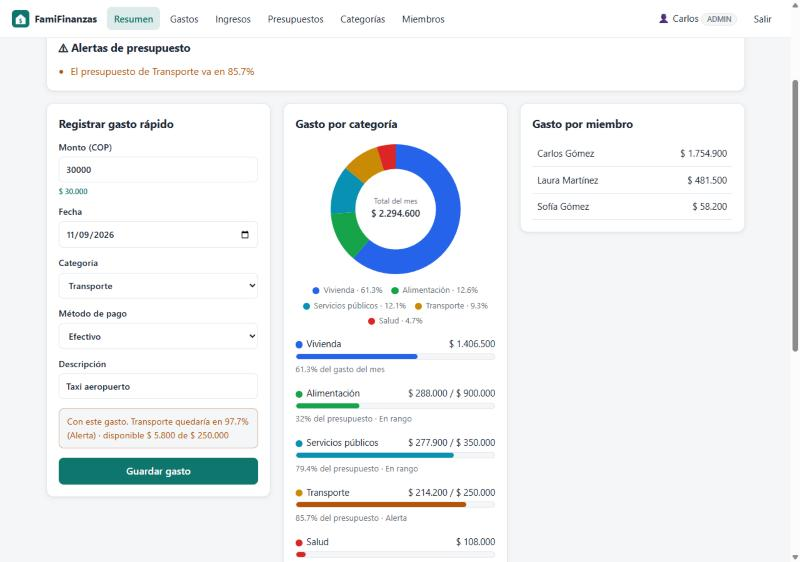
\includegraphics[width=\columnwidth]{figuras/dashboard-ts.jpg}
\caption{Resumen del mes: gráfico \texttt{GraficoCategorias} y simulación del presupuesto de Transporte antes de guardar un gasto (97,7\,\%, Alerta).}
\label{fig:pantalla-dashboard}
\end{figure}

\begin{figure}[!t]
\centering
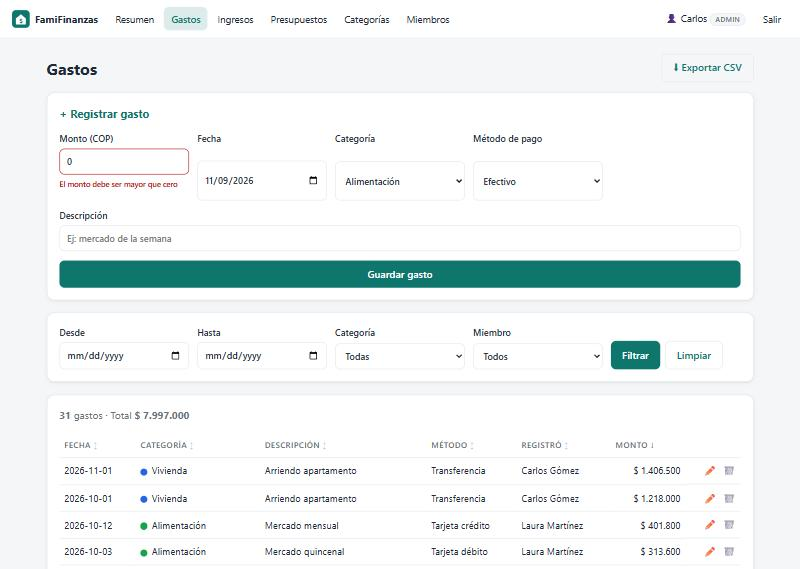
\includegraphics[width=\columnwidth]{figuras/gastos-ts.jpg}
\caption{Gastos: \texttt{ValidadorFormulario} rechaza un monto de 0 y \texttt{TablaOrdenable} ordena por monto descendente.}
\label{fig:pantalla-gastos}
\end{figure}

% =====================================================================
\section{Modelado UML}\label{sec:uml}
Los diagramas siguen la notación UML 2.5.1 \cite{uml251} y reflejan el código TypeScript implementado.

\subsection{Diagrama de casos de uso}
La Fig.~\ref{fig:casos-uso} presenta los actores \emph{Visitante}, \emph{Miembro} y \emph{Administrador} (este último especializa al Miembro) y los casos de uso RF-01 a RF-14. En naranja se destacan los dos casos nuevos que aporta el frontend TypeScript: la simulación del presupuesto, que extiende a \emph{Registrar gasto}, y la visualización del gráfico, que extiende a \emph{Consultar resumen mensual}.

\begin{figure*}[!t]
\centering
\resizebox{0.95\textwidth}{!}{% Diagrama de casos de uso — FamiFinanzas (versión TypeScript)
\begin{tikzpicture}[
  uc/.style={ellipse, draw=teal!60!black, fill=teal!6, thick, minimum width=3.7cm, minimum height=1.0cm,
             align=center, font=\scriptsize, inner sep=0.5pt},
  ucts/.style={uc, draw=orange!75!black, fill=orange!12},
  asoc/.style={thick},
  dep/.style={dashed, -{Stealth[length=2mm]}},
  etq/.style={font=\tiny, fill=white, inner sep=1pt},
]
% Límite del sistema
\draw[thick, rounded corners=4pt, fill=gray!3] (2.6,-2.0) rectangle (17.9,10.1);
\node[anchor=north west, font=\small\bfseries] at (2.7,10.05) {Sistema FamiFinanzas (TypeScript)};

% Actores
\actorUML{V}{0.6,8.0}{Visitante}
\actorUML{M}{0.6,3.2}{Miembro}
\actorUML{A}{19.6,3.6}{Administrador}

% Columna A: casos del miembro
\node[uc] (UC1)  at (5.4,9.0)  {RF-01 Registrar familia\\y administrador};
\node[uc] (UC2)  at (5.4,7.6)  {RF-02 Iniciar sesión};
\node[uc] (UC13) at (5.4,6.2)  {RF-13 Gestionar perfil\\y contraseña};
\node[uc] (UC5)  at (5.4,4.8)  {RF-05 Registrar gasto};
\node[uc] (UC6)  at (5.4,3.4)  {RF-06 Consultar y\\filtrar gastos};
\node[uc] (UC7)  at (5.4,2.0)  {RF-07 Editar / eliminar\\movimientos};
\node[uc] (UC8)  at (5.4,0.6)  {RF-08 Gestionar ingresos};
\node[uc] (UC11) at (5.4,-0.8) {RF-11 Consultar\\resumen mensual};

% Columna B: casos incluidos / extendidos
\node[uc]   (UCJ)  at (10.6,8.3)  {Generar token JWT};
\node[ucts] (UCS)  at (10.6,6.6)  {Simular presupuesto\\(cliente TS)};
\node[uc]   (UC10) at (10.6,4.8)  {RF-10 Generar alerta\\de presupuesto};
\node[uc]   (UC12) at (10.6,3.2)  {RF-12 Exportar\\gastos a CSV};
\node[uc]   (UC14) at (10.6,1.2)  {RF-14 Verificar\\permisos por rol};
\node[ucts] (UCG)  at (10.6,-0.8) {Visualizar gráfico\\(cliente TS)};

% Columna C: casos del administrador
\node[uc] (UC3) at (15.6,6.0) {RF-03 Gestionar\\miembros};
\node[uc] (UC4) at (15.6,3.9) {RF-04 Gestionar\\categorías};
\node[uc] (UC9) at (15.6,1.8) {RF-09 Definir\\presupuestos};

% Asociaciones actor - caso de uso
\draw[asoc] (V-e) -- (UC1.west);
\draw[asoc] (V-e) -- (UC2.west);
\foreach \cu in {UC13,UC5,UC6,UC7,UC8,UC11} \draw[asoc] (M-e) -- (\cu.west);
\foreach \cu in {UC3,UC4,UC9} \draw[asoc] (A-o) -- (\cu.east);

% Generalización de actores: Administrador es un Miembro
\draw[thick, -{Triangle[open, length=3mm, width=3mm]}]
  (A-etq.south) -- (19.6,-2.6) -- (0.6,-2.6) -- (M-etq.south);

% Include / extend
\draw[dep] (UC1) -- node[etq, sloped, above] {\estereotipo{include}} (UCJ);
\draw[dep] (UC2) -- node[etq, sloped, below] {\estereotipo{include}} (UCJ);
\draw[dep] (UCS) -- node[etq, sloped, above] {\estereotipo{extend}} (UC5);
\draw[dep] (UC10) -- node[etq, above, align=center] {\estereotipo{extend}\\{}[gasto $\geq$ 80\,\%]} (UC5);
\draw[dep] (UC12) -- node[etq, above] {\estereotipo{extend}} (UC6);
\draw[dep] (UC7) -- node[etq, sloped, above] {\estereotipo{include}} (UC14);
\draw[dep] (UCG) -- node[etq, above] {\estereotipo{extend}} (UC11);
\draw[dep] (UC11.north east) -- (8.0,-0.2) -- node[etq, sloped, above, pos=0.55] {\estereotipo{include}} (8.0,4.3) -- (UC10.south west);
% Bus de "include" de los casos del administrador hacia RF-14
\draw[thick, dashed] (UC3.west) -- (13.15,6.0) -- (13.15,1.2);
\draw[thick, dashed] (UC4.west) -- (13.15,3.9);
\draw[thick, dashed] (UC9.west) -- (13.15,1.8);
\draw[dep] (13.15,1.2) -- (UC14.east);
\node[etq, rotate=90] at (13.15,5.0) {\estereotipo{include}};

% Leyenda
\node[ucts, minimum width=1.0cm, minimum height=0.45cm] (ley) at (4.1,-2.9) {};
\node[anchor=west, font=\scriptsize] at (ley.east) {Funcionalidad nueva del frontend en TypeScript};
\end{tikzpicture}
}
\caption{Diagrama de casos de uso de FamiFinanzas (versión TypeScript).}
\label{fig:casos-uso}
\end{figure*}

\subsection{Diagrama de componentes}
La Fig.~\ref{fig:componentes} muestra los componentes en tiempo de ejecución. En el navegador se ejecuta el JavaScript generado desde \texttt{client/}; en el servidor, el generado en \texttt{dist/}. El artefacto \texttt{contratos.d.ts} solo existe en tiempo de compilación y es importado con \texttt{import type} por el cliente y por el servidor. La API REST se ofrece como interfaz a clientes externos (Swagger UI, Postman) con autenticación \emph{Bearer}.

\begin{figure*}[!t]
\centering
\resizebox{\textwidth}{!}{% Diagrama de componentes — FamiFinanzas (versión TypeScript)
\begin{tikzpicture}[
  comp/.style={draw, thick, fill=white, minimum width=3.6cm, minimum height=1.05cm, align=center,
               font=\scriptsize, inner sep=3pt},
  paquete/.style={draw, thick, rounded corners=3pt, inner sep=9pt},
  dep/.style={dashed, -{Stealth[length=2mm]}},
  flujo/.style={thick, -{Stealth[length=2.2mm]}},
  etq/.style={font=\tiny, fill=white, inner sep=1pt, align=center},
]
% ---------------- Navegador (cliente) ----------------
\node[comp] (VHTML) at (2.2,10.2)  {Vistas HTML\\(plantillas EJS)};
\node[comp] (MAIN)  at (6.4,10.2)  {main.js\\(de client/main.ts)};
\node[comp] (UI)    at (10.6,10.2) {Componentes UI\\Validador, Simulador\\Gráfico, TablaOrdenable};
\node[comp] (HTTP)  at (14.8,10.2) {ClienteHttp\\(fetch tipado)};
\foreach \cc in {VHTML,MAIN,UI,HTTP} {\iconoComponente{\cc}}
\begin{scope}[on background layer]
  \node[paquete, fill=blue!4, fit=(VHTML)(MAIN)(UI)(HTTP),
        label={[font=\small\bfseries, anchor=south west]north west:Navegador web (JavaScript generado por tsc en public/js)}] {};
\end{scope}
\draw[dep] (VHTML) -- node[etq, above=2pt] {\estereotipo{module}} (MAIN);
\draw[dep] (MAIN) -- node[etq, above=2pt] {monta} (UI);
\draw[dep] (UI) -- node[etq, above=2pt] {usa} (HTTP);

% ---------------- Servidor ----------------
\node[comp] (EXP) at (2.2,7.2)  {Express app\\(app.ts, Helmet)};
\node[comp] (WEB) at (6.4,7.2)  {webRouter\\(web.ts + vistas.ts)};
\node[comp] (MW)  at (10.6,7.2) {Middlewares\\(auth.ts, errores.ts)};
\node[comp] (API) at (14.8,7.2) {apiRouter\\(routes/api/index.ts)};
\node[comp] (DI)  at (2.2,5.0)  {Contenedor DI\\(contenedor.ts)};
\node[comp] (SRV) at (8.5,5.0)  {Servicios\\(AuthService, GastoService...)};
\node[comp] (DOM) at (14.8,3.2) {Dominio\\(Entidad, Movimiento...)};
\node[comp] (REP) at (8.5,3.2)  {Repositorios\\(RepositorioBase$<$E,F$>$)};
\node[comp] (BD)  at (8.5,1.4)  {BaseDatos\\(node:sqlite)};
\foreach \cc in {EXP,WEB,MW,API,DI,SRV,DOM,REP,BD} {\iconoComponente{\cc}}
\begin{scope}[on background layer]
  \node[paquete, fill=teal!5, fit=(EXP)(WEB)(MW)(API)(DI)(SRV)(DOM)(REP)(BD),
        label={[font=\small\bfseries, anchor=north west]south west:Servidor Node.js $\geq$ 22 (dist/)}] {};
\end{scope}

\draw[flujo] (EXP) -- (WEB);
\draw[flujo] ($(EXP.north east)+(-0.4,0)$) |- (14.8,8.1) -- (API.north);
\draw[dep] (WEB) -- node[etq, above=2pt] {usa} (MW);
\draw[dep] (API) -- node[etq, above=2pt] {usa} (MW);
\draw[dep] (WEB.south) -- (SRV.north west);
\draw[dep] (API.south west) -- (SRV.north east);
\draw[dep] (DI) -- node[etq, above=2pt] {\estereotipo{crea}} (SRV);
\draw[dep] (SRV) -- (REP);
\draw[dep] (REP) -- (BD);
\draw[dep] (REP) -- node[etq, above=2pt] {instancia} (DOM);
\draw[dep] (SRV.south east) -- (DOM.north west);

% Base de datos (fuera del proceso)
\node[cylinder, shape border rotate=90, aspect=0.25, draw, thick, fill=gray!8, minimum width=2.6cm, minimum height=1.3cm,
      align=center, font=\scriptsize] (DB) at (8.5,-1.2) {famifinanzas.db\\(SQLite)};
\draw[flujo] (BD) -- node[etq, right=2pt] {SQL parametrizado} (DB);

% Conexiones navegador -> servidor
\draw[flujo] (VHTML) -- node[etq, right=2pt] {HTTP: HTML y formularios\\(cookie JWT httpOnly)} (EXP);
\draw[flujo] (HTTP.south) -- ++(0,-0.75) -| node[etq, pos=0.25, above] {GET /datos/presupuestos (JSON)} (WEB.north);

% Interfaz provista por la API (notación lollipop) y cliente externo
\coordinate (iApi) at (17.5,7.2);
\draw[thick] (API.east) -- ($(iApi)+(-0.16,0)$);
\draw[thick, fill=white] (iApi) circle (0.16);
\node[etq, below=4pt] at (iApi) {REST /api/v1\\(Bearer JWT)};
\node[comp, fill=gray!6] (EXT) at (19.6,5.0) {Cliente de la API\\(Swagger UI / Postman)};
\iconoComponente{EXT}
\draw[dep] (EXT.north) |- ($(iApi)+(0.2,0)$);

% Artefacto con los contratos compartidos (solo tipos)
\node[draw, thick, fill=orange!12, align=center, font=\scriptsize, minimum height=1.0cm] (CON) at (19.6,9.0)
  {\estereotipo{artifact}\\contratos.d.ts};
\draw[dep] (HTTP.east) -| node[etq, pos=0.2, above] {import type} (CON.north);
\draw[dep] (API.north east) -- node[etq, sloped, below] {import type} (CON.south west);
\end{tikzpicture}
}
\caption{Diagrama de componentes: cliente TypeScript, servidor TypeScript por capas y contratos compartidos.}
\label{fig:componentes}
\end{figure*}

\subsection{Diagrama de secuencia}
La Fig.~\ref{fig:secuencia} describe el escenario principal del sistema migrado: registrar un gasto. En la primera fase el componente \texttt{SimuladorPresupuesto} consulta al servidor, autenticado con la cookie, y proyecta el porcentaje de ejecución en el navegador; en la segunda, el formulario se envía, el servidor valida con el esquema tipado, registra el gasto y calcula la alerta RF-10 con la clase \texttt{EjecucionPresupuesto}.

\begin{figure*}[!t]
\centering
\resizebox{\textwidth}{!}{% Diagrama de secuencia — Registrar gasto con simulación de presupuesto en el cliente TS
\begin{tikzpicture}[
  part/.style={draw, thick, fill=teal!8, minimum height=0.9cm, minimum width=2.5cm, align=center, font=\scriptsize},
  msj/.style={semithick, -{Stealth[length=2.4mm, width=1.8mm]}},
  ret/.style={semithick, dashed, -{Stealth[length=2.4mm, width=1.8mm]}},
  txt/.style={font=\scriptsize, above, inner sep=1.5pt, fill=white},
]
\def\fin{-17.3}
% Participantes (x)
\def\xU{0}  \def\xS{3.3} \def\xC{6.6} \def\xW{9.9} \def\xA{12.9} \def\xP{15.9} \def\xG{18.9} \def\xR{21.9}

\actorUML{U}{\xU,0.3}{Usuario}
\node[part, fill=orange!12] (S) at (\xS,0) {:SimuladorPresupuesto\\(navegador)};
\node[part, fill=orange!12] (C) at (\xC,0) {:ClienteHttp\\(navegador)};
\node[part] (W) at (\xW,0) {:webRouter};
\node[part] (A) at (\xA,0) {autenticarWeb};
\node[part] (P) at (\xP,0) {:PresupuestoService};
\node[part] (G) at (\xG,0) {:GastoService};
\node[part] (R) at (\xR,0) {:Repositorios\\+ SQLite};
% Líneas de vida
\foreach \x in {\xU,\xS,\xC,\xW,\xA,\xP,\xG,\xR} \draw[dashed, gray] (\x,-0.6) -- (\x,\fin);

% --- Fase 1: simulación en el cliente (TypeScript en el navegador) ---
\node[draw, fill=orange!8, font=\scriptsize\bfseries, anchor=west] at (-0.6,-1.0) {Fase 1: simulación (cliente TS)};
\draw[msj] (\xU,-1.6) -- node[txt] {1: escribe monto, fecha y categoría} (\xS,-1.6);
\draw[msj] (\xS,-2.3) -- node[txt] {2: obtener$<$EjecucionPresupuestoDTO[]$>$()} (\xC,-2.3);
\draw[msj] (\xC,-3.0) -- node[txt] {3: GET /datos/presupuestos?mes (cookie ff\_token)} (\xW,-3.0);
\draw[msj] (\xW,-3.7) -- node[txt] {4: verificar JWT} (\xA,-3.7);
\draw[ret] (\xA,-4.4) -- node[txt] {5: Usuario (actor)} (\xW,-4.4);
\draw[msj] (\xW,-5.1) -- node[txt] {6: listar(actor, mes)} (\xP,-5.1);
\draw[msj] (\xP,-5.8) -- node[txt] {7: listarPorMes() / totalCategoriaMes()} (\xR,-5.8);
\draw[ret] (\xR,-6.5) -- node[txt] {8: filas tipadas} (\xP,-6.5);
\draw[ret] (\xP,-7.2) -- node[txt] {9: EjecucionPresupuestoDTO[]} (\xW,-7.2);
\draw[ret] (\xW,-7.9) -- node[txt] {10: 200 application/json} (\xC,-7.9);
\draw[ret] (\xC,-8.6) -- node[txt] {11: \{ok: true, datos\}} (\xS,-8.6);
\draw[msj] (\xS,-9.1) -- ++(0.9,0) -- ++(0,-0.5) node[midway, right, font=\scriptsize] {12: proyectar(gastado, monto, límite)} -- (\xS,-9.6);
\draw[ret] (\xS,-10.2) -- node[txt] {13: ``quedaría en 97,7\,\% (Alerta)''} (\xU,-10.2);

% --- Fase 2: registro en el servidor ---
\draw[gray, dash dot] (-0.6,-10.7) -- (22.8,-10.7);
\node[draw, fill=teal!8, font=\scriptsize\bfseries, anchor=west] at (-0.6,-11.1) {Fase 2: registro (servidor TS)};
\draw[msj] (\xU,-11.7) -- node[txt, pos=0.75] {14: POST /gastos (formulario)} (\xW,-11.7);
\draw[msj] (\xW,-12.2) -- ++(0.9,0) -- ++(0,-0.5) node[midway, right, font=\scriptsize] {15: validar(esquemas.gasto) : EntradaGasto} -- (\xW,-12.7);
\draw[msj] (\xW,-13.3) -- node[txt, pos=0.7] {16: crear(actor, datos)} (\xG,-13.3);
\draw[msj] (\xG,-14.0) -- node[txt] {17: INSERT gasto} (\xR,-14.0);
\draw[msj] (\xG,-14.7) -- node[txt] {18: alertaCategoria()} (\xP,-14.7);
\draw[ret] (\xP,-15.4) -- node[txt] {19: Alerta | null} (\xG,-15.4);
\draw[ret] (\xG,-16.1) -- node[txt, pos=0.7] {20: ResultadoGasto \{gasto, alerta\}} (\xW,-16.1);
\draw[ret] (\xW,-16.8) -- node[txt, pos=0.3] {21: 302 /dashboard + mensaje flash} (\xU,-16.8);

% Marco del diagrama (sd)
\draw[thick] (-1.0,2.2) rectangle (23.2,\fin-0.3);
\node[draw, thick, fill=white, anchor=north west, font=\scriptsize\bfseries] at (-1.0,2.2) {sd Registrar gasto con simulación de presupuesto};
\end{tikzpicture}
}
\caption{Diagrama de secuencia: registrar un gasto con simulación del presupuesto en el cliente TypeScript.}
\label{fig:secuencia}
\end{figure*}

\subsection{Diagramas de clases}
La Fig.~\ref{fig:clases-dominio} presenta el modelo de dominio: herencia desde \texttt{Entidad<TDTO>}, la abstracción \texttt{Movimiento}, la realización de interfaces, la composición \texttt{Familia}--\texttt{Usuario}/\texttt{Movimiento} y las enumeraciones. La Fig.~\ref{fig:clases-capas} muestra las capas de acceso a datos y de servicios, donde los genéricos permiten reutilizar la lógica común; y la Fig.~\ref{fig:clases-err} la jerarquía de errores y los componentes del cliente.

\begin{figure*}[p]
\centering
\resizebox{\textwidth}{!}{% Diagrama de clases del dominio (src/dominio) — FamiFinanzas TypeScript
\begin{tikzpicture}[clases]
% Columnas
\def\cA{0} \def\cB{4.3} \def\cC{8.6} \def\cD{12.9} \def\cE{17.2}

% ---------- Fila 1: interfaces y objetos calculados ----------
\interfaz{Actor}{\cA,0}{\estereotipo{interface}\\\textbf{Actor}}
  {+ id: number \{readonly\}\\+ familiaId: number \{readonly\}\\+ esAdmin(): boolean}
\interfaz{Serializable}{\cB,0}{\estereotipo{interface}\\\textbf{Serializable$<$TDTO$>$}}
  {+ toJSON(): TDTO}
\interfaz{Modificable}{\cC,0}{\estereotipo{interface}\\\textbf{Modificable}}
  {+ puedeSerModificadoPor(actor: Actor): boolean}
\clase{Alerta}{\cD,0}{\textbf{Alerta}}
  {+ categoria: string\\- ejecucion: EjecucionPresupuesto\\- contexto?: ContextoAlerta}
  {+ \textit{get} estado(): EstadoPresupuesto\\+ \textit{get} mensaje(): string\\+ toJSON(): AlertaDTO}
\clase{Resumen}{\cE,0}{\textbf{ResumenMensual}}
  {+ mes: string\\+ totalIngresos: number\\+ totalGastos: number\\+ porCategoria: TotalCategoriaDTO[]\\+ porMiembro: TotalMiembroDTO[]\\- \#alertas: Alerta[]}
  {+ \textit{get} balance(): number\\+ toJSON(): ResumenMensualDTO}

% ---------- Fila 2: raíz de la jerarquía ----------
\clase{Entidad}{\cB,-2.6}{{\tiny\estereotipo{abstract}}\\\textit{\textbf{Entidad$<$TDTO$>$}}}
  {+ id: number \{readonly\}}
  {+ \textit{toJSON(): TDTO}\\+ esIgualA(otra: Entidad): boolean}

% ---------- Fila 3: entidades ----------
\clase{Usuario}{\cA,-5.6}{\textbf{Usuario}}
  {+ familiaId: number\\+ nombre: string\\+ email: string\\+ rol: Rol\\+ activo: boolean\\+ creadoEn: string\\- \#passwordHash: string}
  {+ esAdmin(): boolean\\+ \textit{get} hashContrasena(): string\\+ toJSON(): UsuarioDTO}
\clase{Familia}{\cB,-5.6}{\textbf{Familia}}
  {+ nombre: string\\+ moneda: string = "COP"\\+ creadoEn: string}
  {+ toJSON(): FamiliaDTO}
\clase{Movimiento}{\cC,-5.6}{{\tiny\estereotipo{abstract}}\\\textit{\textbf{Movimiento$<$TDTO$>$}}}
  {+ monto: number \{$>$ 0\}\\+ fecha: string\\+ descripcion: string\\+ usuario: RefUsuarioDTO\\+ creadoEn: string}
  {+ \textit{get tipo(): TipoMovimiento}\\+ \textit{get} mes(): string\\+ puedeSerModificadoPor(a): boolean\\\# camposBase(): MovimientoDTO}
\clase{Categoria}{\cD,-5.6}{\textbf{Categoria}}
  {+ \underline{COLOR\_POR\_DEFECTO}\\+ nombre: string\\+ color: string\\+ activo: boolean}
  {+ \textit{get} referencia(): RefCategoriaDTO\\+ toJSON(): CategoriaDTO}
\clase{Presupuesto}{\cE,-5.6}{\textbf{Presupuesto}}
  {+ mes: string \estereotipo{AAAA-MM}\\+ montoLimite: number\\+ categoria: RefCategoriaDTO}
  {+ evaluar(gastado, umbral): EjecucionPresupuesto\\+ conEjecucion(gastado, umbral)\\+ toJSON(): PresupuestoDTO}

% ---------- Fila 4 ----------
\interfaz{Rol}{\cA,-11.2}{\estereotipo{enumeration}\\\textbf{Rol}}{ADMIN\\MIEMBRO}
\clase{Ingreso}{\cB,-11.2}{\textbf{Ingreso}}
  {+ fuente: string}
  {+ \textit{get} tipo(): 'INGRESO'\\+ toJSON(): IngresoDTO}
\clase{Gasto}{\cC,-11.2}{\textbf{Gasto}}
  {+ \underline{ENCABEZADO\_CSV}\\+ metodoPago: MetodoPago\\+ categoria: RefCategoriaDTO}
  {+ \textit{get} tipo(): 'GASTO'\\+ aFilaCsv(): (string | number)[]\\+ toJSON(): GastoDTO}
\interfaz{MetodoPago}{\cD,-11.2}{\estereotipo{enumeration}\\\textbf{MetodoPago}}{EFECTIVO\\TARJETA\_DEBITO\\TARJETA\_CREDITO\\TRANSFERENCIA}
\clase{Ejecucion}{\cE,-11.2}{\textbf{EjecucionPresupuesto}}
  {+ estado: EstadoPresupuesto\\+ porcentaje: number | null}
  {- constructor() \{privado\}\\+ \underline{calcular(total, limite, umbral)}\\+ \textit{get} requiereAlerta(): boolean\\+ mensajePara(categoria): string}

% ---------- Fila 5 ----------
\interfaz{Exportable}{\cC,-15.0}{\estereotipo{interface}\\\textbf{ExportableCsv}}{+ aFilaCsv(): (string | number)[]}
\interfaz{Estado}{\cE,-15.2}{\estereotipo{enumeration}\\\textbf{EstadoPresupuesto}}{OK\\ALERTA\\EXCEDIDO\\SIN\_PRESUPUESTO}

% ---------- Coordenadas auxiliares ----------
\coordinate (yComp) at (0,-6.7);
\coordinate (yLim)  at (0,-6.5);
\coordinate (yMP)   at (0,-12.0);
\coordinate (yAl)   at (0,-0.9);

% ---------- Relaciones ----------
\draw[realiza] (Entidad.north) -- (Serializable.south);
% Herencia de Entidad (bus)
\def\bus{-4.75}
\draw[thick] (\cA,-5.6) -- (\cA,\bus) -- (\cE,\bus) -- (\cE,-5.6);
\foreach \x in {\cB,\cC,\cD} \draw[thick] (\x,-5.6) -- (\x,\bus);
\draw[herencia] (\cB,\bus) -- (Entidad.south);
% Realizaciones de interfaces
\draw[realiza] ({\cA-0.9},-5.6) -- ($(Actor.south)+(-0.9,0)$);
\draw[realiza] ({\cC+1.0},-5.6) -- ($(Modificable.south)+(1.0,0)$);
% Gasto e Ingreso heredan de Movimiento
\draw[herencia] (Gasto.north) -- (Movimiento.south);
\draw[herencia] (Ingreso.north) |- ($(Movimiento.south)+(-0.6,-0.45)$) -- ($(Movimiento.south)+(-0.6,0)$);
\draw[realiza] (Gasto.south) -- (Exportable.north);
% Asociaciones
\draw[asociacion] ($(Gasto.north)+(1.3,0)$) |- ({\cD-1.0},-10.55) -- node[rol, right, pos=0.5] {clasificado en \quad 1} ($(Categoria.south)+(-1.0,0)$);
\draw[asociacion] (Gasto.east |- yMP) -- (MetodoPago.west |- yMP);
\draw[asociacion] (Presupuesto.west |- yLim) -- node[rol, above] {limita} node[rol, pos=0.85, below] {1} (Categoria.east |- yLim);
\draw[depende] (Presupuesto.south) -- node[rol, right] {\estereotipo{crea}} (Ejecucion.north);
\draw[asociacion] (Ejecucion.south) -- (Estado.north);
\draw[asociacion] (Usuario.south) -- (Rol.north);
% Composición: la familia es dueña de sus usuarios y movimientos
\draw[composicion] (Familia.west |- yComp) -- node[rol, above, pos=0.7] {1..*} (Usuario.east |- yComp);
\draw[composicion] (Familia.east |- yComp) -- node[rol, above, pos=0.7] {0..*} (Movimiento.west |- yComp);
% Resumen agrega alertas
\draw[agregacion] (Resumen.west |- yAl) -- node[rol, above, pos=0.7] {0..*} (Alerta.east |- yAl);
% Lollipops: Alerta y ResumenMensual también realizan Serializable
\foreach \n in {Alerta,Resumen} {
  \draw[thick] (\n.north) -- ++(0,0.35) coordinate (lp\n);
  \draw[thick, fill=white] ($(lp\n)+(0,0.14)$) circle (0.14);
  \node[rol, right] at ($(lp\n)+(0.15,0.14)$) {Serializable};
}
\end{tikzpicture}
}
\caption{Diagrama de clases del dominio (\texttt{src/dominio}). Los nombres en cursiva son abstractos; \# indica miembro protegido o campo privado de ECMAScript.}
\label{fig:clases-dominio}
\end{figure*}

\begin{figure*}[p]
\centering
\resizebox{\textwidth}{!}{% Diagrama de clases de las capas de acceso a datos y servicios — FamiFinanzas TypeScript
\begin{tikzpicture}[clases]
\def\cA{0} \def\cB{4.3} \def\cC{8.6} \def\cD{12.9} \def\cE{17.2}

% ---------------- Repositorios ----------------
\clase{RB}{\cC,0}{{\tiny\estereotipo{abstract}}\\\textit{\textbf{RepositorioBase$<$TEntidad, TFila$>$}}}
  {\# bd: BaseDatos \{readonly\}}
  {\# \textit{mapear(fila: TFila): TEntidad}\\\# uno(sql, ...params): TEntidad | null\\\# varios(sql, ...params): TEntidad[]\\\# ejecutar(sql, ...params): ResultadoEscritura}
\clase{RF}{\cA,-4.8}{\textbf{FamiliaRepository}}{\mbox{}}{+ crear(nombre): Familia\\+ buscarPorId(id): Familia | null}
\clase{RU}{\cB,-4.8}{\textbf{UsuarioRepository}}{\mbox{}}{+ buscarPorEmail(email)\\+ contarAdminsActivos(fam): number\\+ actualizar(id, CambiosUsuario)}
\clase{RC}{\cC,-4.8}{\textbf{CategoriaRepository}}{\mbox{}}{+ listar(fam, opciones): Categoria[]\\+ tieneMovimientos(id): boolean}
\clase{RP}{\cD,-4.8}{\textbf{PresupuestoRepository}}{\mbox{}}{+ listarPorMes(fam, mes)\\+ buscarPorCategoriaMes(...)}
\clase{RM}{\cE,-4.8}{{\tiny\estereotipo{abstract}}\\\textit{\textbf{MovimientoRepository$<$T extends Movimiento, TFila$>$}}}
  {\# \textit{tabla: 'gastos' | 'ingresos'}\\\# \textit{alias: 'g' | 'i'}\\\# \textit{select: string}}
  {\# filtrosAdicionales(c): ClausulaWhere\\+ listar(fam, filtro): ResultadoListado$<$T$>$\\+ listarTodos(fam, criterios): T[]\\+ buscar(id, fam): T | null}
\clase{RG}{\cD,-10.6}{\textbf{GastoRepository}}{\# tabla = 'gastos'}{+ crear(fam, usr, EntradaGasto): Gasto\\+ totalCategoriaMes(...): number\\\# filtrosAdicionales(c) \estereotipo{override}}
\clase{RI}{\cE,-10.6}{\textbf{IngresoRepository}}{\# tabla = 'ingresos'}{+ crear(fam, usr, EntradaIngreso): Ingreso}

\def\busR{-4.15}
\draw[thick] (\cA,-4.8) -- (\cA,\busR) -- (\cE,\busR) -- (\cE,-4.8);
\foreach \x in {\cB,\cD} \draw[thick] (\x,-4.8) -- (\x,\busR);
\draw[herencia] (\cC,-4.8) -- (RB.south);
\draw[herencia] (RG.north) |- ($(RM.south)+(-0.5,-0.4)$) -- ($(RM.south)+(-0.5,0)$);
\draw[herencia] (RI.north) -- (RM.south -| RI.north);

% ---------------- Servicios ----------------
\clase{SA}{\cA,-15.0}{\textbf{AuthService}}{- \#hashFicticio: string}{+ registrar(EntradaRegistro): Promise$<$Sesion$>$\\+ login(EntradaLogin): Promise$<$Sesion$>$\\+ verificarToken(t): PayloadToken}
\clase{SC}{\cC,-15.0}{\textbf{CategoriaService}}{\mbox{}}{+ obtenerActiva(actor, id): Categoria\\+ eliminar(actor, id): ResultadoEliminacion}
\clase{SP}{\cD,-15.0}{\textbf{PresupuestoService}}{- cfg: Configuracion}{+ listar(actor, mes)\\+ crear(actor, EntradaPresupuesto)\\+ alertaCategoria(...): Alerta | null}
\clase{SM}{\cE,-15.0}{{\tiny\estereotipo{abstract}}\\\textit{\textbf{MovimientoService$<$T, R extends MovimientoRepository$>$}}}
  {\# repositorio: R\\\# \textit{recurso: string}}
  {+ listar(actor, filtro): Pagina$<$T$>$\\+ obtener(actor, id): T\\+ eliminar(actor, id): void\\\# verificarPropiedad(actor, m)}
\clase{SU}{\cA,-20.4}{\textbf{UsuarioService}}{\mbox{}}{+ crear(actor, datos): Promise$<$Usuario$>$\\+ actualizar(actor, id, cambios)}
\clase{SR}{\cB,-20.4}{\textbf{ReporteService}}{\mbox{}}{+ resumenMensual(actor, mes): ResumenMensual}
\clase{SG}{\cD,-20.4}{\textbf{GastoService}}{\# recurso = 'Gasto'}{+ crear(actor, datos): ResultadoGasto\\+ actualizar(actor, id, datos)\\+ exportarCsv(actor, criterios): string}
\clase{SI}{\cE,-20.4}{\textbf{IngresoService}}{\# recurso = 'Ingreso'}{+ crear(actor, datos): Ingreso\\+ actualizar(actor, id, datos)}

% Herencia de servicios
\draw[herencia] (SG.north) |- ($(SM.south)+(-0.5,-0.4)$) -- ($(SM.south)+(-0.5,0)$);
\draw[herencia] (SI.north) -- (SM.south -| SI.north);

% Dependencias inyectadas por el constructor (contenedor.ts)
\coordinate (yCat) at (0,-15.8);
\draw[asociacion] (SM.east) -- ++(0.6,0) |- node[rol, right, pos=0.25] {\#repositorio: R} (RM.east);
\draw[asociacion] ($(SG.north)+(-1.0,0)$) -- node[rol, left] {presupuestos} ($(SP.south)+(-1.0,0)$);
\draw[asociacion] (SP.west |- yCat) -- (SC.east |- yCat);
\draw[asociacion] (SP.north) -- node[rol, right] {gastos} (RG.south -| SP.north);
\draw[asociacion] (SC.north) -- node[rol, right, pos=0.4] {categorias} (RC.south -| SC.north);
\draw[asociacion] (SA.north) -- node[rol, right, pos=0.4] {familias, usuarios} (RF.south -| SA.north);
\draw[asociacion] (SU.north) -- node[rol, right] {auth} (SA.south -| SU.north);
\end{tikzpicture}
}
\caption{Diagrama de clases de las capas de repositorios y servicios: genéricos, clases abstractas y dependencias inyectadas por constructor.}
\label{fig:clases-capas}
\end{figure*}

\begin{figure*}[!t]
\centering
\resizebox{\textwidth}{!}{% Diagrama de clases: jerarquía de errores (backend) y componentes del frontend (client/)
\begin{tikzpicture}[clases, clase/.append style={text width=2.5cm}]
\def\xa{0} \def\xb{2.9} \def\xc{5.8} \def\xd{8.7} \def\xe{11.6} \def\xf{14.5}

% ---------------- Errores (src/utils/errores.ts) ----------------
\node[font=\small\bfseries, anchor=west] at (-1.4,1.0) {(a) Jerarquía de errores del backend};
\simple{Error}{\xf,0}{\estereotipo{ECMAScript}\\\textbf{Error}}{+ name: string\\+ message: string}
\clase{App}{\xc+1.45,0}{\textbf{AppError}}
  {+ status: number\\+ codigo: string\\+ detalles?: DetalleErrorDTO[]}
  {+ aRespuesta(): ErrorApiDTO}
\simple{E1}{\xa,-3.2}{\textbf{ValidacionError}}{400 VALIDACION}
\simple{E2}{\xb,-3.2}{\textbf{NoAutenticadoError}}{401 NO\_AUTENTICADO}
\simple{E3}{\xc,-3.2}{\textbf{ProhibidoError}}{403 PROHIBIDO}
\simple{E4}{\xd,-3.2}{\textbf{UsuarioInactivoError}}{403 USUARIO\_INACTIVO}
\simple{E5}{\xe,-3.2}{\textbf{NoEncontradoError}}{404 NO\_ENCONTRADO}
\simple{E6}{\xf,-3.2}{\textbf{ConflictoError}}{409 CONFLICTO}
\draw[herencia] (App.east |- Error.west) -- (Error.west);
\def\busE{-2.55}
\draw[thick] (\xa,-3.2) -- (\xa,\busE) -- (\xf,\busE) -- (\xf,-3.2);
\foreach \x in {\xb,\xc,\xd,\xe} \draw[thick] (\x,-3.2) -- (\x,\busE);
\draw[herencia] ({\xc+1.45},\busE) -- (App.south);

% ---------------- Frontend (client/) ----------------
\node[font=\small\bfseries, anchor=west] at (-1.4,-5.6) {(b) Componentes del frontend TypeScript};
\clase{Comp}{\xc+1.45,-6.4}{{\tiny\estereotipo{abstract}}\\\textit{\textbf{Componente$<$E extends HTMLElement$>$}}}
  {\# raiz: E \{readonly\}}
  {+ \textit{montar(): void}}
\clase{Http}{\xf,-6.4}{\textbf{ClienteHttp}}
  {- \#cache: Map$<$string, Promise$>$\\- base: string}
  {+ obtener$<$T$>$(ruta, params): Promise$<$ Resultado$<$T$>$ $>$\\+ limpiarCache(): void}
\simple{Res}{\xe-0.9,-6.4}{\estereotipo{type}\\\textbf{Resultado$<$T$>$}}{\{ok: true, datos: T\}\\| \{ok: false, status, error\}}

\clase{C1}{\xa,-10.6}{\textbf{ValidadorFormulario}}{- \#mensajes: Map}{- validarCampo(c): boolean}
\clase{C2}{\xb,-10.6}{\textbf{VistaPreviaMonto}}{- \#salida: HTMLElement}{- actualizar(): void}
\clase{C3}{\xc,-10.6}{\textbf{AvisoFlash}}{+ \underline{DURACION\_MS}}{- ocultar(): void}
\clase{C4}{\xd,-10.6}{\textbf{TablaOrdenable}}{\mbox{}}{- ordenar(th, i, tipo)}
\clase{C5}{\xe,-10.6}{\textbf{GraficoCategorias}}{- \#sectores: Sector[]}{- dibujar(resaltado)\\- sectorEn(e): Sector | null}
\clase{C6}{\xf,-10.6}{\textbf{SimuladorPresupuesto}}{- \#consulta: number}{- simular(): Promise$<$void$>$}

\def\busC{-9.85}
\draw[thick] (\xa,-10.6) -- (\xa,\busC) -- (\xf,\busC) -- (\xf,-10.6);
\foreach \x in {\xb,\xc,\xd,\xe} \draw[thick] (\x,-10.6) -- (\x,\busC);
\draw[herencia] ({\xc+1.45},\busC) -- (Comp.south);
\draw[asociacion] ($(C6.north)+(0.9,0)$) -- node[rol, right] {usa} ($(Http.south)+(0.9,0)$);
\draw[depende] (Http.west |- Res.east) -- node[rol, above] {devuelve} (Res.east);
\end{tikzpicture}
}
\caption{Diagrama de clases: (a) jerarquía de errores del backend; (b) componentes del frontend TypeScript (además: \texttt{ConfirmacionAccion}, \texttt{MenuMovil} y \texttt{EnvioUnico}).}
\label{fig:clases-err}
\end{figure*}

% =====================================================================
\section{Resultados y verificación}\label{sec:resultados}
\subsection{Pruebas automatizadas}
Las pruebas se migraron a TypeScript y se ejecutan sobre el código transpilado. Las 26 pruebas de integración de la API y las 3 de las vistas web del Taller~2 pasan sin cambios en sus aserciones, lo que confirma que la migración preservó el comportamiento observable. Se agregaron 11 pruebas unitarias de la jerarquía de clases (herencia, polimorfismo, encapsulamiento, objetos de valor y errores) y una prueba de los endpoints del frontend que verifica el contrato JSON y el escape del JSON incrustado en la página (Tabla~\ref{tab:pruebas}).

\begin{table}[!t]
\centering
\caption{Resultado de \texttt{npm test} (Node.js 22.17)}
\label{tab:pruebas}
\footnotesize
\begin{tabular}{@{}lrr@{}}
\toprule
\textbf{Archivo} & \textbf{Pruebas} & \textbf{Aprobadas} \\
\midrule
tests/api.test.ts (integración API) & 26 & 26 \\
tests/web.test.ts (vistas y /datos) & 4 & 4 \\
tests/dominio.test.ts (unitarias POO) & 11 & 11 \\
\midrule
\textbf{Total} & \textbf{41} & \textbf{41} \\
\bottomrule
\end{tabular}
\end{table}

\subsection{Métricas de la migración}
La Tabla~\ref{tab:metricas} compara ambas versiones. El aumento de líneas se explica por las anotaciones de tipo, las interfaces y la documentación TSDoc, y por el nuevo frontend; a cambio, la lógica duplicada de repositorios y servicios se eliminó mediante herencia. El rendimiento (RNF-05) se midió con 10\,000 gastos en la base de datos: el percentil 95 fue de 6,2\,ms al listar gastos, 3,6\,ms al registrarlos y 8,7\,ms en el resumen mensual, muy por debajo del objetivo de 300\,ms.

\begin{table}[!t]
\centering
\caption{Comparación entre la versión JavaScript y la TypeScript}
\label{tab:metricas}
\footnotesize
\begin{tabularx}{\columnwidth}{@{}Xrr@{}}
\toprule
\textbf{Métrica} & \textbf{JS} & \textbf{TS} \\
\midrule
Archivos del backend (\texttt{src/}) & 25 & 46 \\
Líneas del backend (con comentarios) & 1\,432 & 2\,844 \\
Archivos / líneas del frontend & 1 / 25 & 12 / 612 \\
Clases (backend + frontend) & 1 & 47 \\
Interfaces / alias de tipo / \texttt{enum} & 0 / 0 / 0 & 62 / 29 / 3 \\
Pruebas automatizadas & 29 & 41 \\
Errores de tipos al compilar (\texttt{tsc}) & --- & 0 \\
\bottomrule
\end{tabularx}
\end{table}

\subsection{Ventajas observadas de TypeScript}
\begin{itemize}
\item \textbf{Detección temprana}: errores de forma de datos, parámetros y nulos aparecen al compilar y en el editor, no en producción.
\item \textbf{Contratos únicos}: \texttt{contratos.d.ts} y \texttt{z.infer} mantienen sincronizados API, servidor y cliente.
\item \textbf{Diseño orientado a objetos verificable}: \texttt{abstract}, \texttt{implements}, \texttt{override} y los genéricos convierten el diagrama de clases en código que el compilador hace cumplir \cite{gamma1994}.
\item \textbf{Mantenibilidad}: el autocompletado y la refactorización segura reducen el costo de cambio; los \texttt{Record<Enum, \ldots>} obligan a cubrir cada valor nuevo.
\item \textbf{Sin costo en ejecución}: el JavaScript generado es equivalente al escrito a mano y el rendimiento no cambió.
\end{itemize}

% =====================================================================
\section{Conclusiones}\label{sec:conclusiones}
La migración de FamiFinanzas a TypeScript se completó en el backend y en el frontend sin alterar el comportamiento de la API, como lo demuestran las 29 pruebas originales que siguen pasando. El cambio no fue solo sintáctico: el modelo pasó de objetos literales a una jerarquía de clases con interfaces, clases abstractas, genéricos y encapsulamiento real, que coincide con el diagrama de clases y que el compilador hace cumplir. La configuración estricta y el uso de \texttt{import type} producen, tras la transpilación, JavaScript ES2022 limpio. En el cliente, TypeScript permitió construir componentes reutilizables que consumen la API con contratos compartidos y resultados tipados, lo que incorporó nuevas funcionalidades (simulación de presupuesto y gráfico) con menor riesgo. La principal lección es que una migración incremental respaldada por pruebas existentes permite adoptar TypeScript de forma segura, y que su mayor beneficio aparece cuando se aprovechan los tipos para expresar el diseño y no solo para anotar variables.

\begin{thebibliography}{00}
\bibitem{tshandbook} Microsoft, ``The TypeScript Handbook,'' 2025. [En línea]. Disponible: \url{https://www.typescriptlang.org/docs/handbook/intro.html}
\bibitem{bierman2014} G. Bierman, M. Abadi y M. Torgersen, ``Understanding TypeScript,'' en \emph{Proc. ECOOP 2014}, LNCS, vol.~8586, Springer, 2014, pp.~257--281.
\bibitem{gao2017} Z. Gao, C. Bird y E. T. Barr, ``To type or not to type: Quantifying detectable bugs in JavaScript,'' en \emph{Proc. 39th Int. Conf. Software Engineering (ICSE)}, 2017, pp.~758--769.
\bibitem{tsconfig} Microsoft, ``TSConfig Reference,'' 2025. [En línea]. Disponible: \url{https://www.typescriptlang.org/tsconfig}
\bibitem{rfc7519} M. Jones, J. Bradley y N. Sakimura, ``JSON Web Token (JWT),'' IETF, RFC 7519, may. 2015.
\bibitem{nodesqlite} OpenJS Foundation, ``SQLite --- Node.js v22 Documentation.'' [En línea]. Disponible: \url{https://nodejs.org/docs/latest-v22.x/api/sqlite.html}
\bibitem{zod} C. McDonnell, ``Zod: TypeScript-first schema validation with static type inference.'' [En línea]. Disponible: \url{https://zod.dev}
\bibitem{fowler2002} M. Fowler, \emph{Patterns of Enterprise Application Architecture}. Boston, MA, EE.~UU.: Addison-Wesley, 2002.
\bibitem{gamma1994} E. Gamma, R. Helm, R. Johnson y J. Vlissides, \emph{Design Patterns: Elements of Reusable Object-Oriented Software}. Reading, MA, EE.~UU.: Addison-Wesley, 1994.
\bibitem{ecma262} Ecma International, \emph{ECMA-262: ECMAScript 2022 Language Specification}, 13.\textsuperscript{a} ed., jun. 2022.
\bibitem{mdnmodules} Mozilla, ``JavaScript modules,'' MDN Web Docs. [En línea]. Disponible: \url{https://developer.mozilla.org/en-US/docs/Web/JavaScript/Guide/Modules}
\bibitem{uml251} Object Management Group, \emph{OMG Unified Modeling Language (OMG UML), Version 2.5.1}, formal/17-12-05, dic. 2017.
\end{thebibliography}

\end{document}
